\documentclass{article}
\usepackage{fullpage}

%load needed packages
\usepackage{graphicx}
\usepackage{array}
\usepackage{booktabs}
\usepackage[utf8]{inputenc}
\usepackage[T1]{fontenc}
\usepackage{url}
\usepackage[spanish]{babel} % Paquete para el idioma español
\usepackage{float}  % Necesario para [H]
\usepackage{listings}
\usepackage{xcolor}

\definecolor{codegreen}{HTML}{5AB2FF}
\definecolor{morado}{HTML}{AD88C6}
\definecolor{BG}{HTML}{EEEEEE}
\definecolor{azul}{HTML}{4D869C}
\definecolor{sqlblue}{HTML}{FF8C00} % Color para las palabras clave SQL

% Estilo para DDL
\lstdefinestyle{ddlstyle}{
	language=SQL,
	backgroundcolor=\color{BG},
	commentstyle=\color{codegreen},
	basicstyle=\ttfamily\small,
	keywordstyle=\color{azul},
	stringstyle=\color{morado},
	showstringspaces=false,
	breaklines=true,
	frame=shadowbox,
	numbers=left,
	numberstyle=\tiny\color{gray},
	captionpos=b,
}

% Estilo para SQL
\lstdefinestyle{sqlstyle}{
	language=SQL,
	backgroundcolor=\color{BG},
	commentstyle=\color{codegreen},
	basicstyle=\ttfamily\small,
	keywordstyle=\color{sqlblue}, % Color diferente para palabras clave SQL
	stringstyle=\color{morado},
	showstringspaces=false,
	breaklines=true,
	frame=shadowbox,
	numbers=left,
	numberstyle=\tiny\color{gray},
	captionpos=b,
}

\begin{document}
	
	
	
	% Portada
	\begin{titlepage}
		\centering
		\vspace*{3cm}
		
		% Título destacado
		{\Huge \textbf{Visualización de Datos (Power BI)}\\[0.5cm]}
		
		% Espacio y logotipo (si lo tienes, por ejemplo el logo de tu universidad)
		\vspace{2cm}
		
\includegraphics[width=0.3\textwidth]{images/uma_logo.jpg}\\[1cm]
		
		% Nombre del autor

		{\LARGE \textbf{Marta Cuevas Rodríguez}\\[0.5cm]}
		{\large \textit{Almacenes De Datos}\\
			Universidad de Málaga\\
		}
		
		\vfill
		
		% Fecha en la parte inferior de la página
		{\large Enero 2025}
	\end{titlepage}
	
	% indice
	\tableofcontents
	
	\newpage
\section{Introducción}
\label{sec:introduccion}




\section{Objetivos}
\label{sec:objetivos}



\begin{itemize}
aaakakañ
ajaaa
\end{itemize}










\section{Creación del proyecto en Power BI}
 explicar ... subo fotos y hay que explicar pasos 
 
\subsection{Pasos Iniciales}
----- cambiar pies de fotos

\begin{figure}[H]
	\begin{center} 
		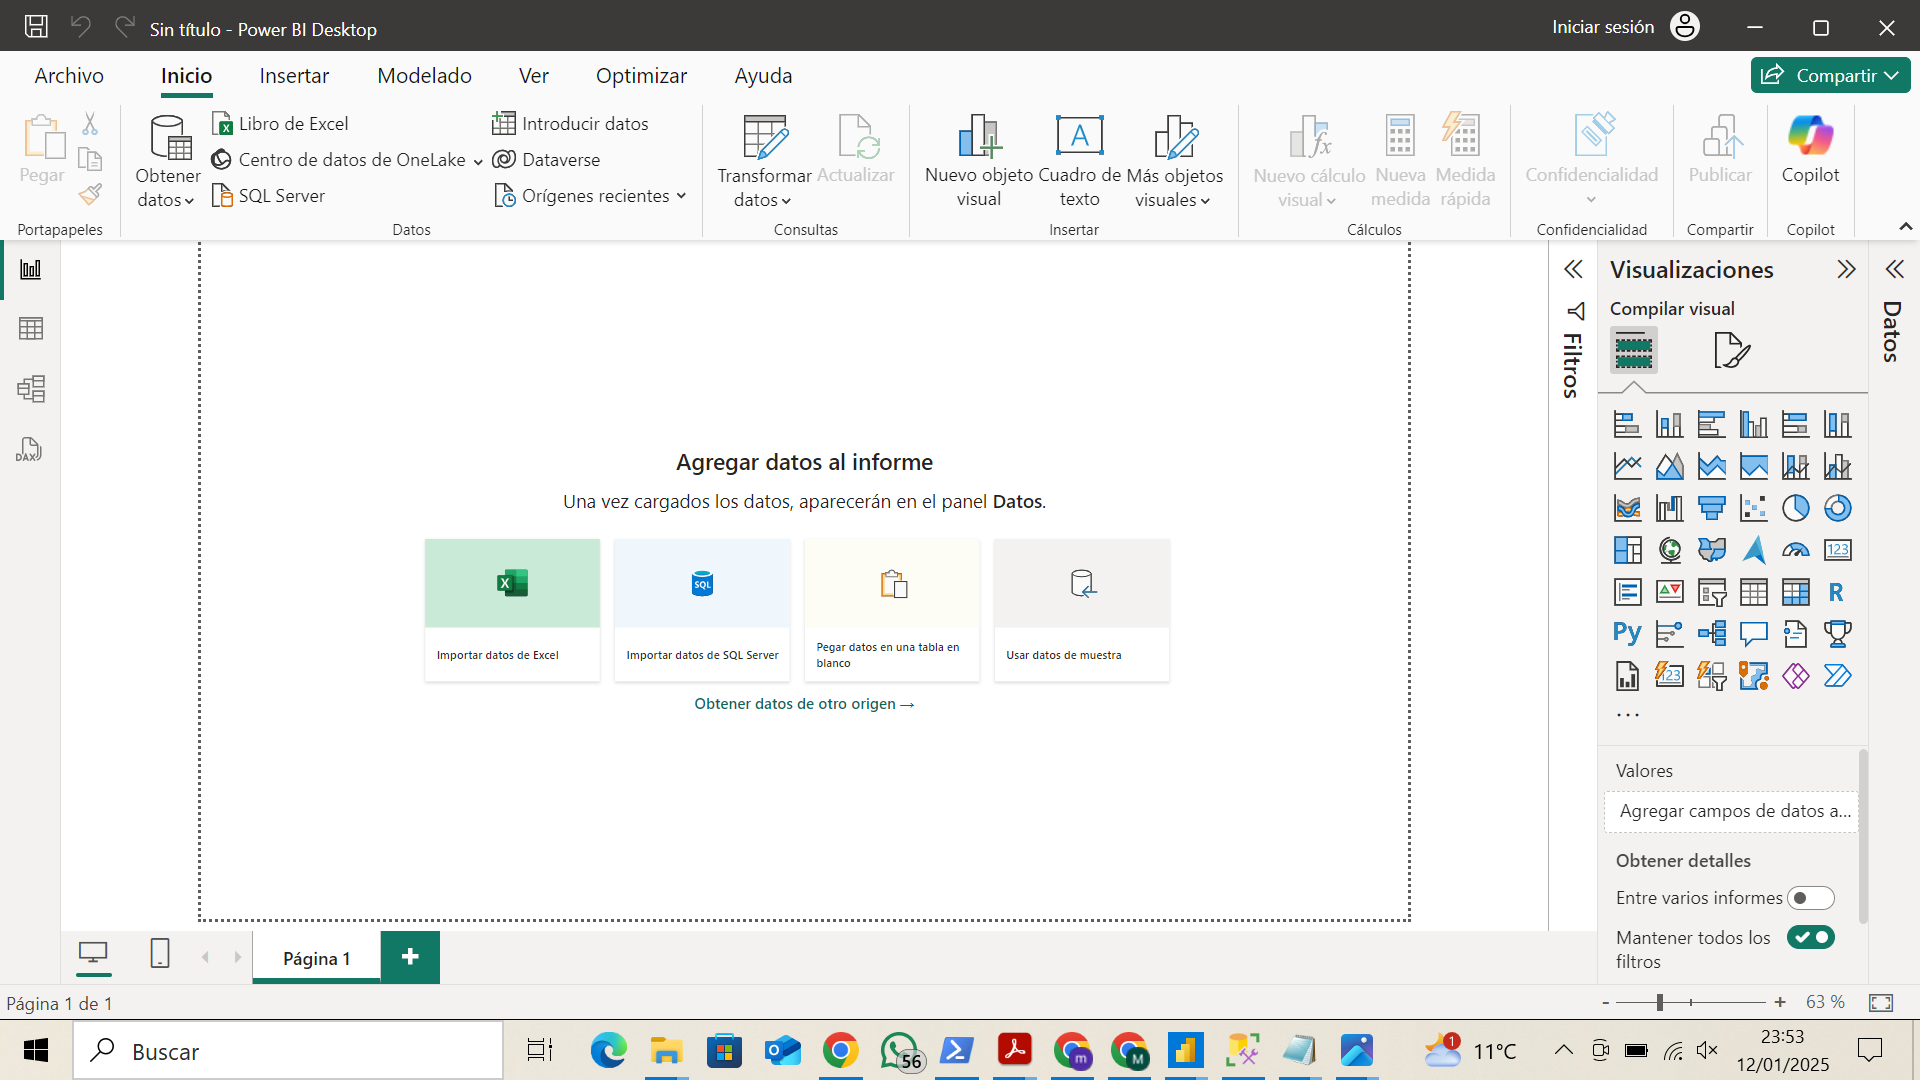
\includegraphics[width=\textwidth]{images/tutorial1.png}
		\caption{Creación de un nuevo proyecto multidimensional en Visual Studio.}
		\label{fig:tutorial1}
	\end{center}
\end{figure}



\begin{figure}[H]
	\begin{center} 
		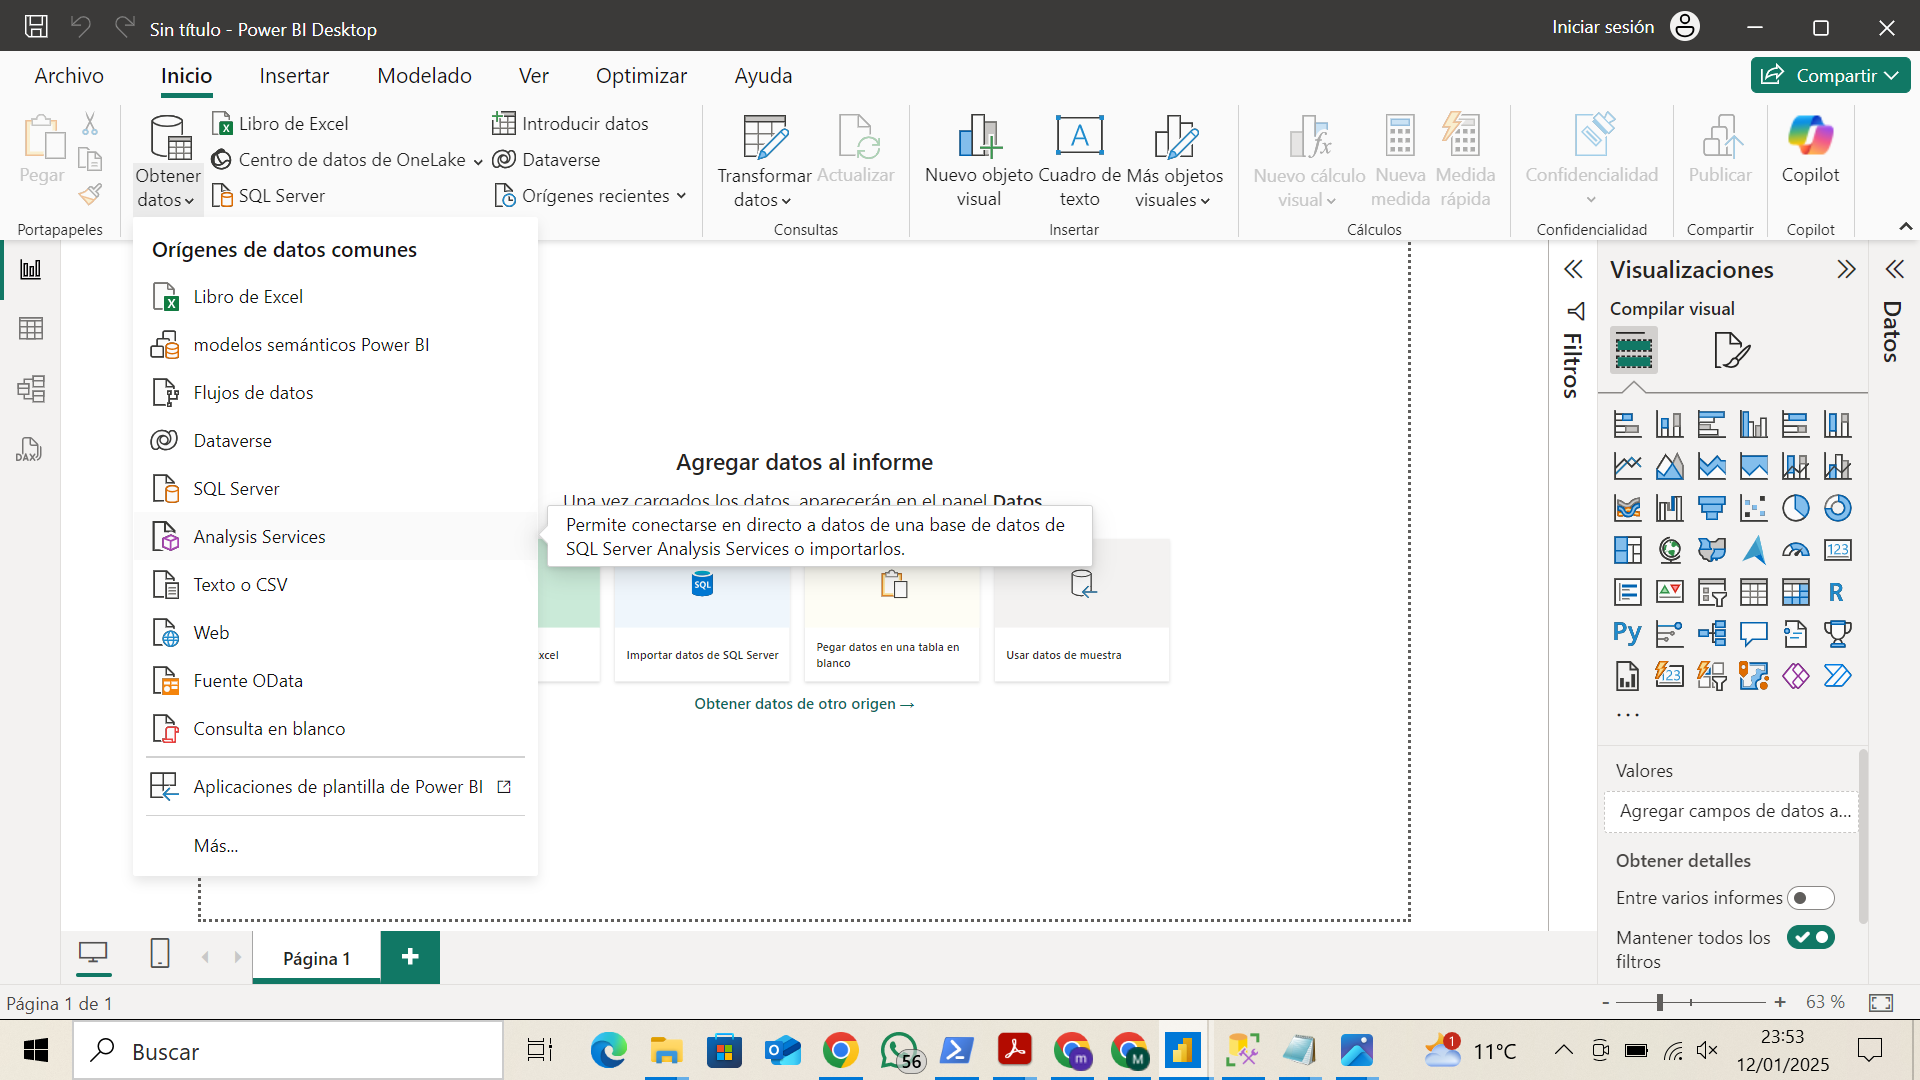
\includegraphics[width=\textwidth]{images/tutorial2.png}
		\caption{Creación de un nuevo proyecto multidimensional en Visual Studio.}
		\label{fig:tutorial2}
	\end{center}
\end{figure}

\begin{figure}[H]
	\begin{center} 
		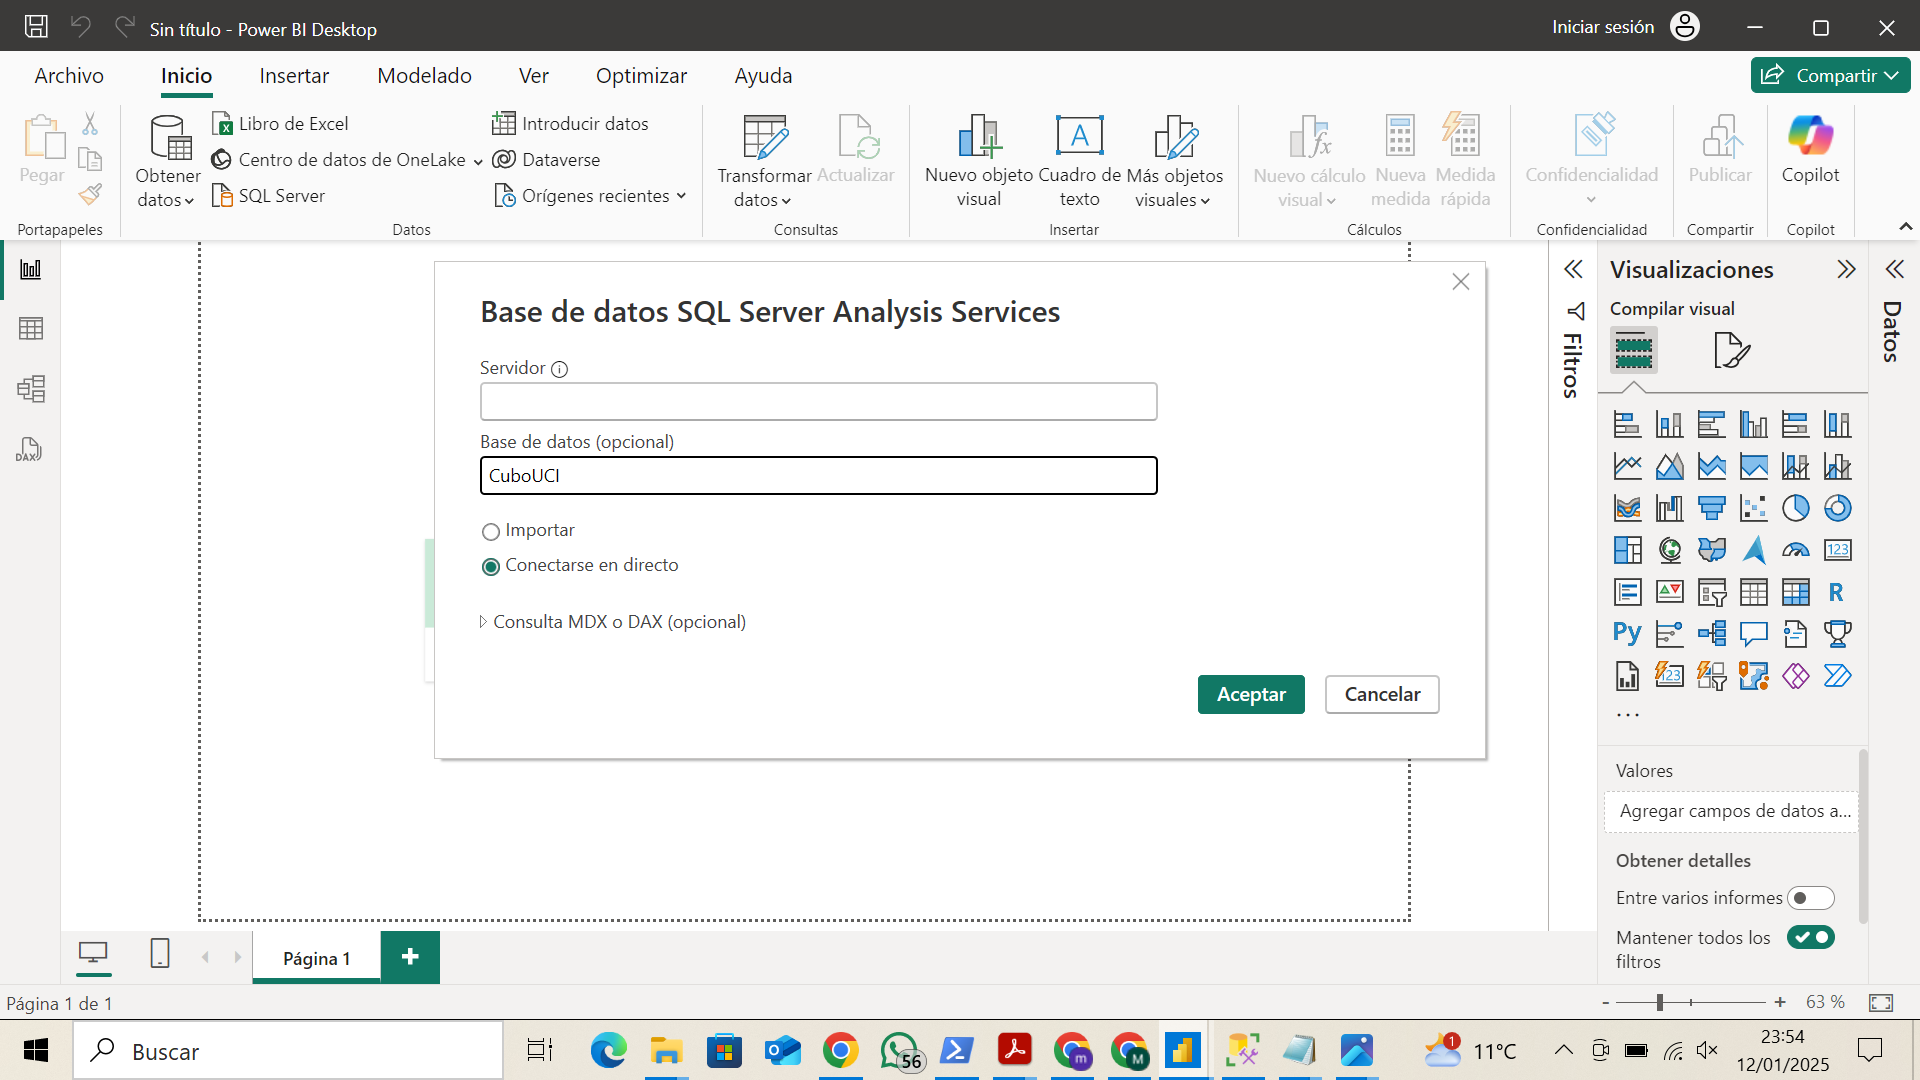
\includegraphics[width=\textwidth]{images/tutorial3.png}
		\caption{Creación de un nuevo proyecto multidimensional en Visual Studio.}
		\label{fig:tutorial3}
	\end{center}
\end{figure}

\begin{figure}[H]
	\begin{center} 
		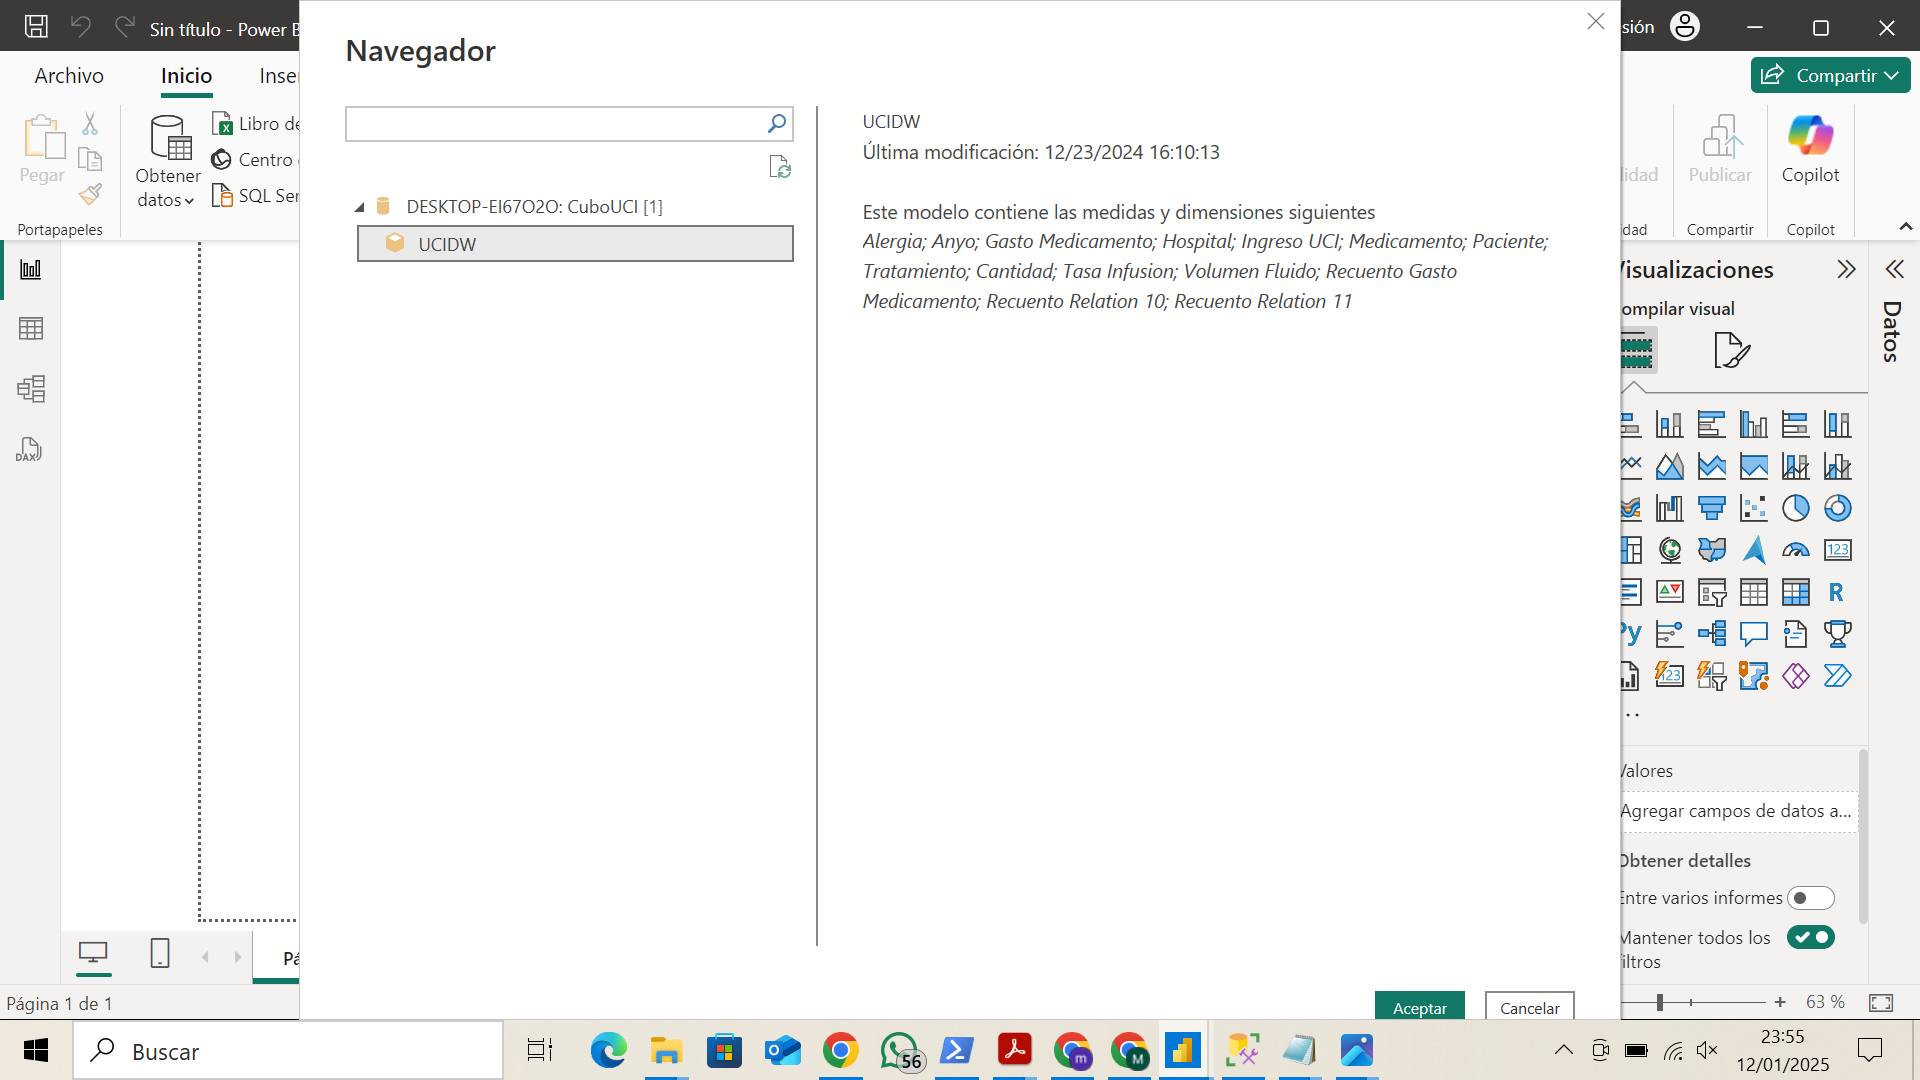
\includegraphics[width=\textwidth]{images/tutorial4.png}
		\caption{Creación de un nuevo proyecto multidimensional en Visual Studio.}
		\label{fig:tutorial4}
	\end{center}
\end{figure}

\begin{figure}[H]
	\begin{center} 
		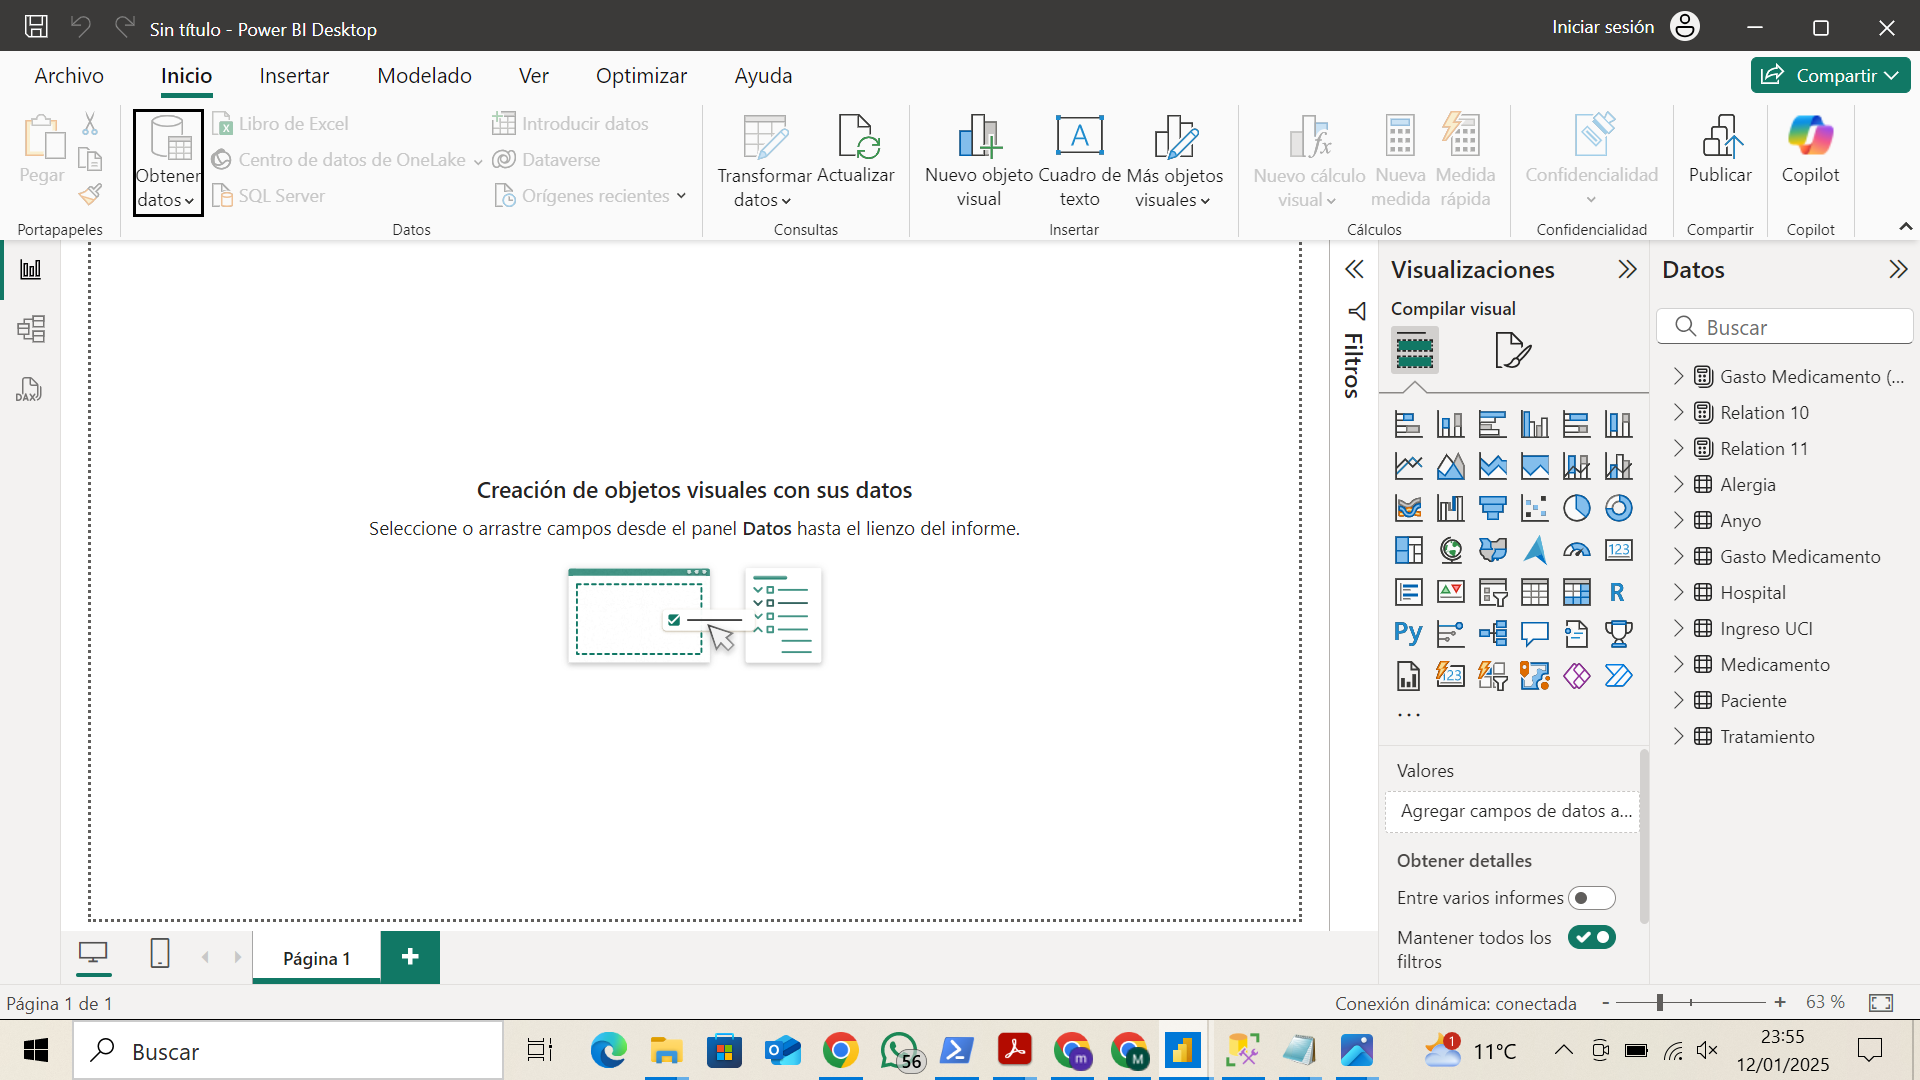
\includegraphics[width=\textwidth]{images/tutorial5.png}
		\caption{Creación de un nuevo proyecto multidimensional en Visual Studio.}
		\label{fig:tutorial5}
	\end{center}
\end{figure}

\begin{figure}[H]
	\begin{center} 
		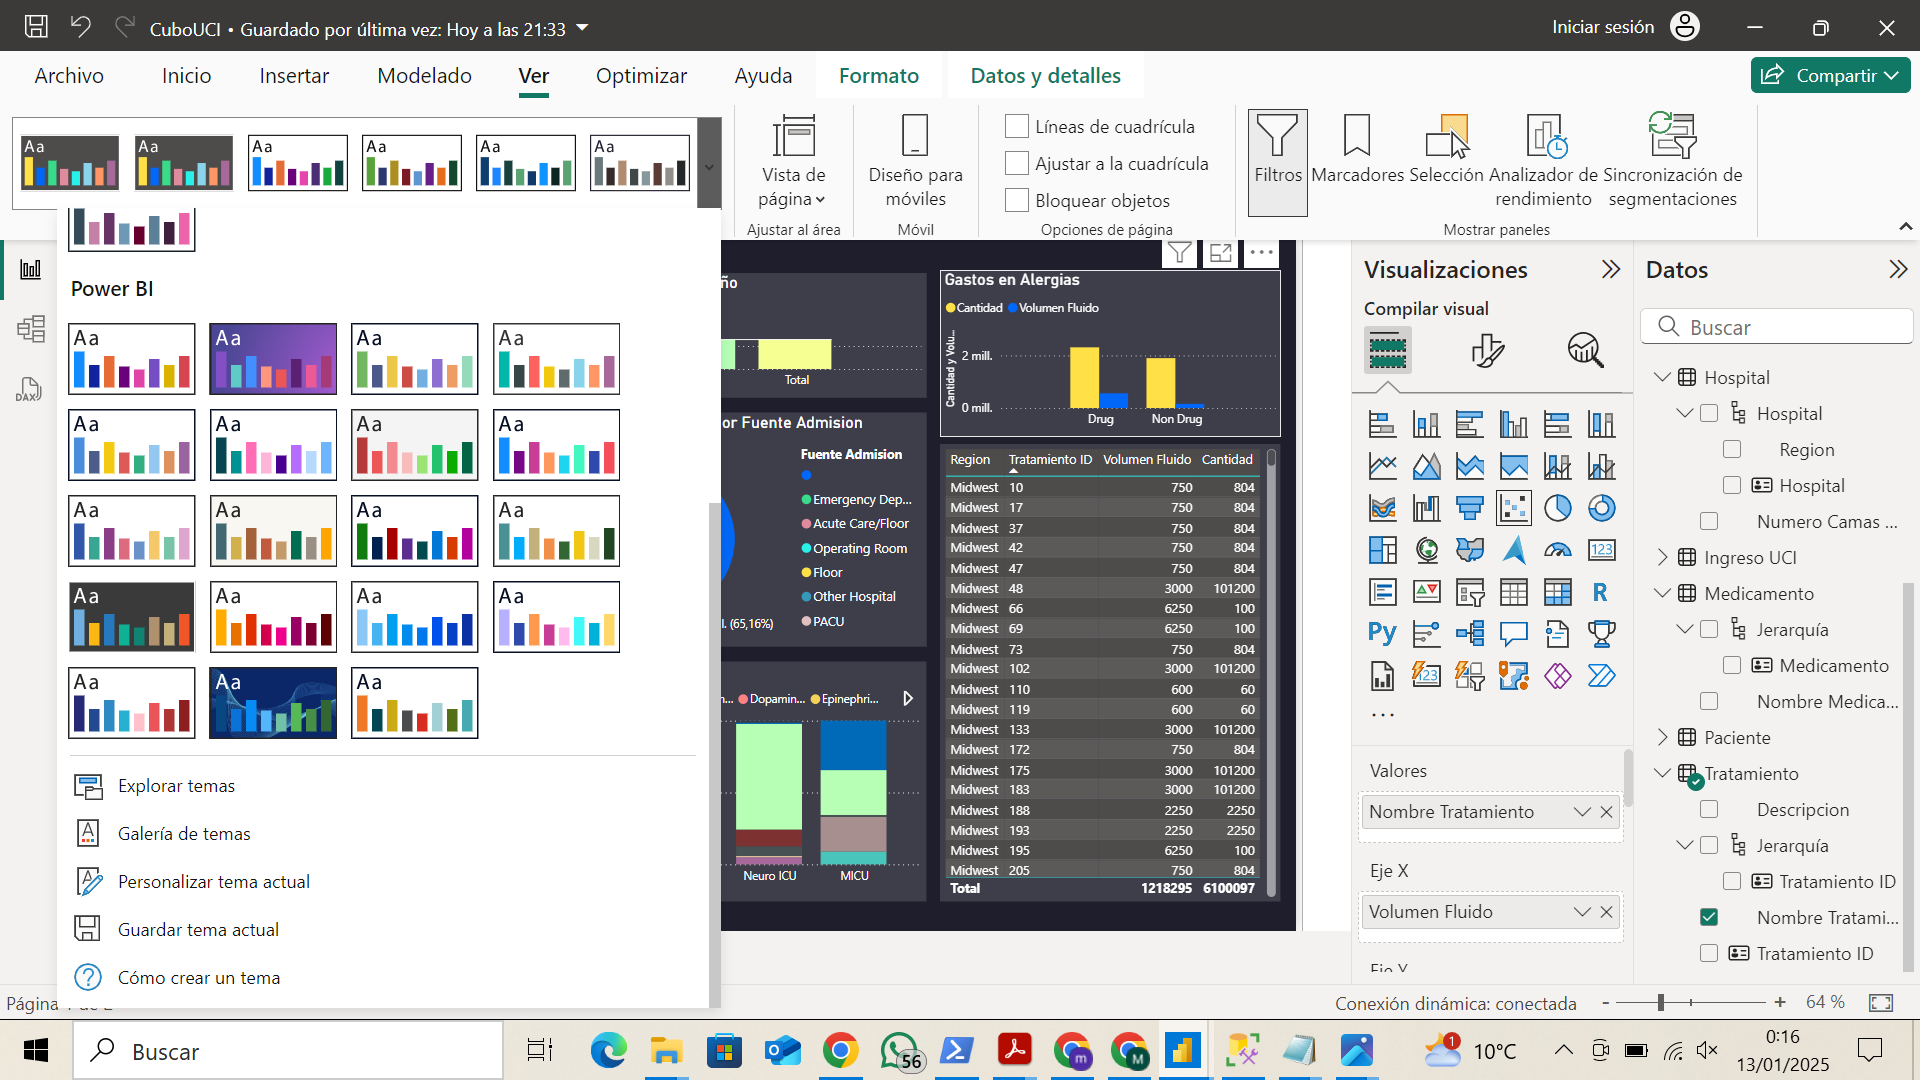
\includegraphics[width=\textwidth]{images/tutorial6.png}
		\caption{Creación de un nuevo proyecto multidimensional en Visual Studio.}
		\label{fig:tutorial6}
	\end{center}
\end{figure}



	
	
	
	
	
	
	
	
	
	
\section{Graficas}
	------
\subsection{Gráfica 1 titulos y tal ponerlos}

\textbf{Ranking de Hospitales según Volumen de Fluido}
\\

explicar y cambiar titulos
\\

\begin{figure}[H]
	\begin{center} 
		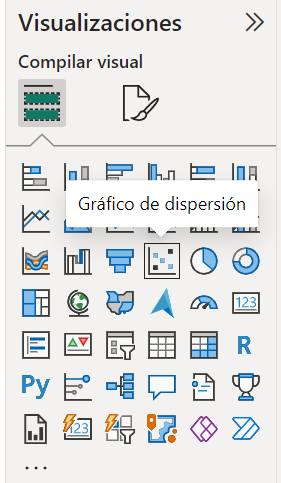
\includegraphics[width=0.35\linewidth]{images/tipo1.png}
		\caption{Creación de un nuevo proyecto multidimensional en Visual Studio.}
		\label{fig:tipo1}
	\end{center}
\end{figure}

\begin{figure}[H]
	\begin{center} 
		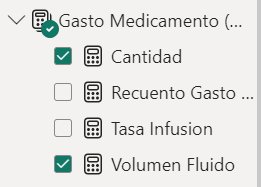
\includegraphics[width=0.4\linewidth]{images/seleccion1-1.png}
		\caption{Creación de un nuevo proyecto multidimensional en Visual Studio.}
		\label{fig:seleccion11}
	\end{center}
\end{figure}

\begin{figure}[H]
	\begin{center} 
		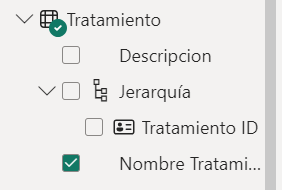
\includegraphics[width=0.4\linewidth]{images/seleccion1-2.png}
		\caption{Creación de un nuevo proyecto multidimensional en Visual Studio.}
		\label{fig:seleccion12}
	\end{center}
\end{figure}

\begin{figure}[H]
	\begin{center} 
		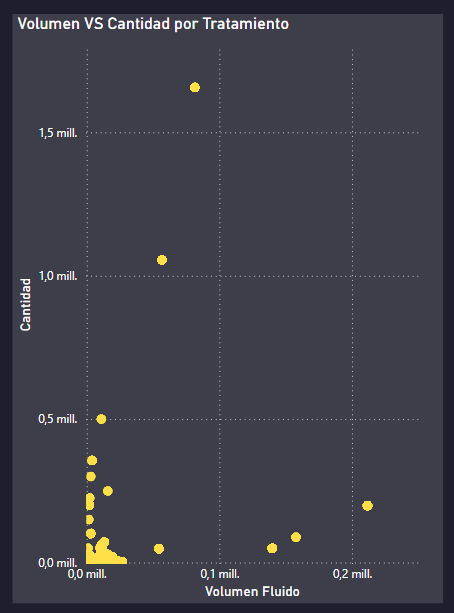
\includegraphics[width=0.5\linewidth]{images/tabla1.png}
		\caption{Creación de un nuevo proyecto multidimensional en Visual Studio.}
		\label{fig:tabla1}
	\end{center}
\end{figure}

\begin{lstlisting}[style=ddlstyle, label=lst:consulta1,caption=Consulta 1: Ranking de Hospitales según Volumen de Fluido]


SELECT
	{
		[Measures].[Volumen Fluido],
		[Measures].[Cantidad]
	} ON COLUMNS,
	NONEMPTY(
	[Tratamiento].[Nombre Tratamiento].Children
	) ON ROWS
FROM 
	[UCIDW]

\end{lstlisting}

\begin{figure}[H]
	\centering
	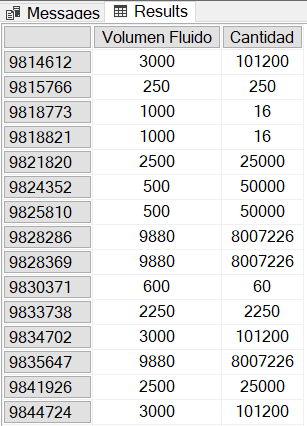
\includegraphics[width=0.35\linewidth]{images/consulta1.png}
	\caption{Resultados de la consulta 1: Ranking de Hospitales según Volumen de Fluido}
	\label{fig:consulta1}
\end{figure}


\subsection{Gráfica 2}

\textbf{Ranking de Hospitales según Volumen de Fluido}
\\

explicar y cambiar titulos
\\

\begin{figure}[H]
	\begin{center} 
		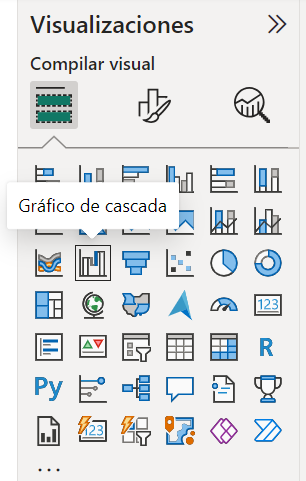
\includegraphics[width=0.35\linewidth]{images/tipo2.png}
		\caption{Creación de un nuevo proyecto multidimensional en Visual Studio.}
		\label{fig:tipo2}
	\end{center}
\end{figure}

\begin{figure}[H]
	\begin{center} 
		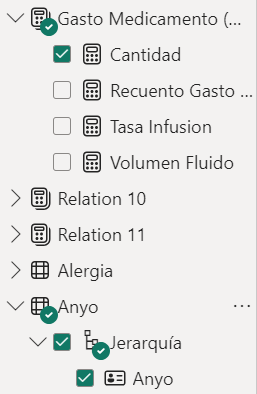
\includegraphics[width=0.4\linewidth]{images/seleccion2.png}
		\caption{Creación de un nuevo proyecto multidimensional en Visual Studio.}
		\label{fig:seleccion2}
	\end{center}
\end{figure}


\begin{figure}[H]
	\begin{center} 
		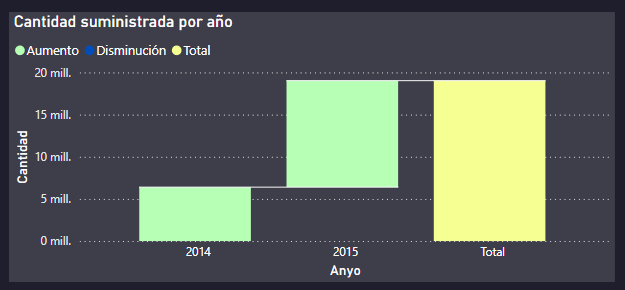
\includegraphics[width=0.7\linewidth]{images/tabla2.png}
		\caption{Creación de un nuevo proyecto multidimensional en Visual Studio.}
		\label{fig:tabla2}
	\end{center}
\end{figure}

\begin{lstlisting}[style=ddlstyle, label=lst:consulta1,caption=Consulta 1: Ranking de Hospitales según Volumen de Fluido]
	
	

WITH 
	MEMBER [Anyo].[Jerarquia].[Total] AS 
	AGGREGATE(
	[Anyo].[Jerarquia].[Anyo].Members
	)
SELECT
	[Measures].[Cantidad] ON COLUMNS,
	{
		nonempty([Anyo].[Jerarquia].[Anyo].Members),
	[Anyo].[Jerarquia].[Total]
	} ON ROWS
FROM
	[UCIDW]
	
\end{lstlisting}

\begin{figure}[H]
	\centering
	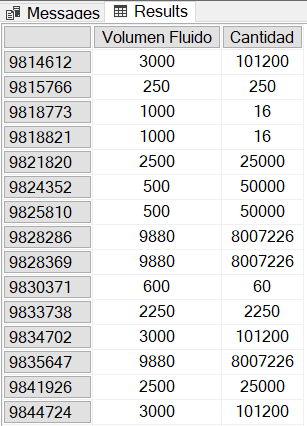
\includegraphics[width=0.35\linewidth]{images/consulta1.png}
	\caption{Resultados de la consulta 1: Ranking de Hospitales según Volumen de Fluido}
	\label{fig:consulta2}
\end{figure}

\subsection{Gráfica 3}

\textbf{Ranking de Hospitales según Volumen de Fluido}
\\

explicar y cambiar titulos
\\

\begin{figure}[H]
	\begin{center} 
		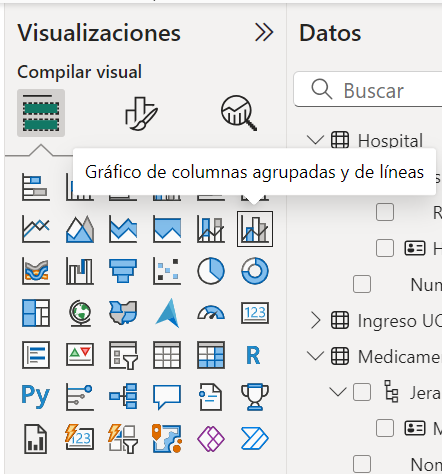
\includegraphics[width=0.35\linewidth]{images/tipo3.png}
		\caption{Creación de un nuevo proyecto multidimensional en Visual Studio.}
		\label{fig:tipo3}
	\end{center}
\end{figure}

\begin{figure}[H]
	\begin{center} 
		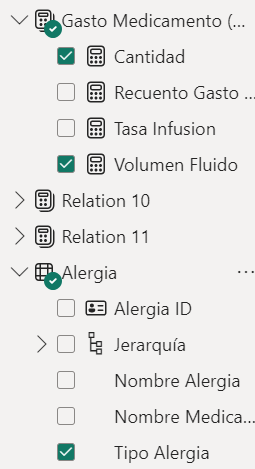
\includegraphics[width=0.35\linewidth]{images/seleccion3.png}
		\caption{Creación de un nuevo proyecto multidimensional en Visual Studio.}
		\label{fig:seleccion3}
	\end{center}
\end{figure}


\begin{figure}[H]
	\begin{center} 
		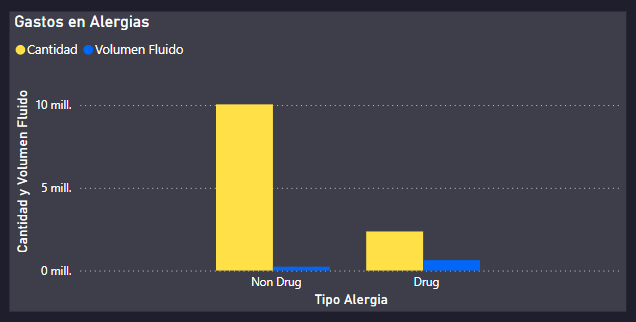
\includegraphics[width=0.7\linewidth]{images/tabla3.png}
		\caption{Creación de un nuevo proyecto multidimensional en Visual Studio.}
		\label{fig:tabla3}
	\end{center}
\end{figure}

\begin{lstlisting}[style=ddlstyle, label=lst:consulta1,caption=Consulta 1: Ranking de Hospitales según Volumen de Fluido]
	
	
SELECT
	{
		[Measures].[Volumen Fluido],
		[Measures].[Cantidad]
	} ON COLUMNS,
NONEMPTY(
	[Alergia].[Tipo Alergia].Children
	) ON ROWS
FROM 
	[UCIDW]
	
\end{lstlisting}

\begin{figure}[H]
	\centering
	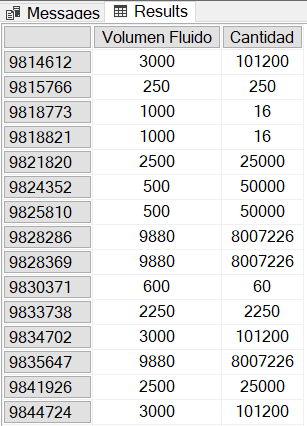
\includegraphics[width=0.35\linewidth]{images/consulta1.png}
	\caption{Resultados de la consulta 1: Ranking de Hospitales según Volumen de Fluido}
	\label{fig:consulta3}
\end{figure}

\subsection{Gráfica 4}

\textbf{Ranking de Hospitales según Volumen de Fluido}
\\

explicar y cambiar titulos
\\

\begin{figure}[H]
	\begin{center} 
		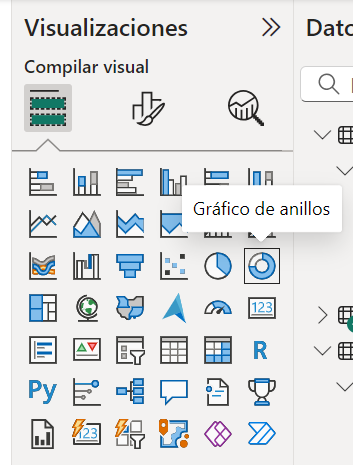
\includegraphics[width=0.35\linewidth]{images/tipo4.png}
		\caption{Creación de un nuevo proyecto multidimensional en Visual Studio.}
		\label{fig:tipo4}
	\end{center}
\end{figure}

\begin{figure}[H]
	\begin{center} 
		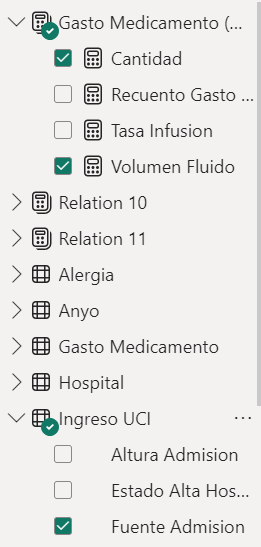
\includegraphics[width=0.35\linewidth]{images/seleccion4.png}
		\caption{Creación de un nuevo proyecto multidimensional en Visual Studio.}
		\label{fig:seleccion4}
	\end{center}
\end{figure}


\begin{figure}[H]
	\begin{center} 
		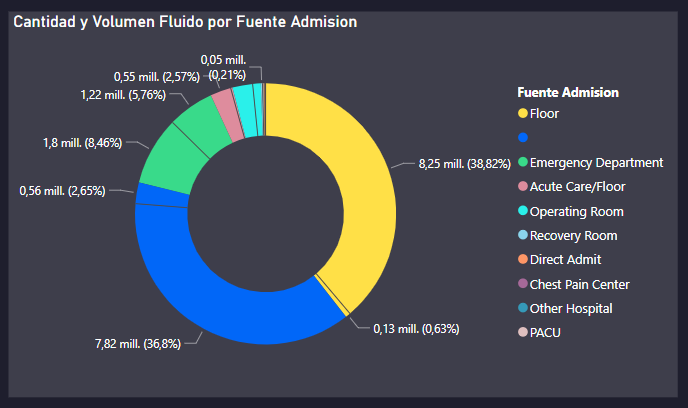
\includegraphics[width=0.7\linewidth]{images/tabla4.png}
		\caption{Creación de un nuevo proyecto multidimensional en Visual Studio.}
		\label{fig:tabla4}
	\end{center}
\end{figure}

\begin{lstlisting}[style=ddlstyle, label=lst:consulta1,caption=Consulta 1: Ranking de Hospitales según Volumen de Fluido]
	
	
SELECT
	{
		[Measures].[Volumen Fluido],
		[Measures].[Cantidad]
	} ON COLUMNS,
	NONEMPTY(
		[Ingreso UCI].[Fuente Admision].Children
	) ON ROWS
FROM 
	[UCIDW]
	
\end{lstlisting}

\begin{figure}[H]
	\centering
	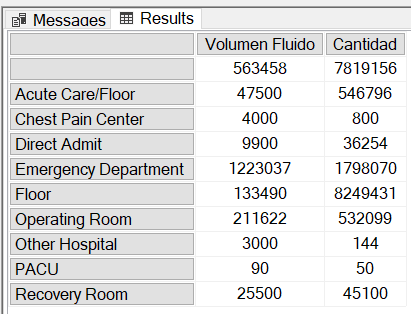
\includegraphics[width=0.45\linewidth]{images/consulta4.png}
	\caption{Resultados de la consulta 1: Ranking de Hospitales según Volumen de Fluido}
	\label{fig:consulta4}
\end{figure}

\subsection{Gráfica 5}

\textbf{Ranking de Hospitales según Volumen de Fluido}
\\

explicar y cambiar titulos
\\

\begin{figure}[H]
	\begin{center} 
		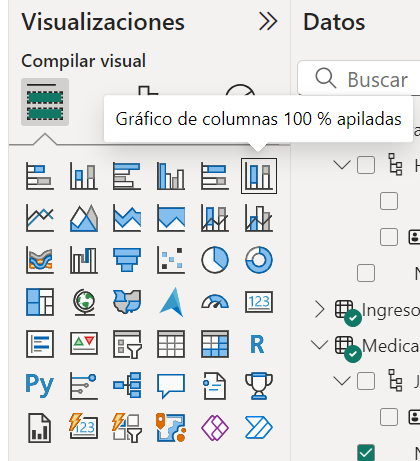
\includegraphics[width=0.35\linewidth]{images/tipo5.png}
		\caption{Creación de un nuevo proyecto multidimensional en Visual Studio.}
		\label{fig:tipo5}
	\end{center}
\end{figure}

\begin{figure}[H]
	\begin{center} 
		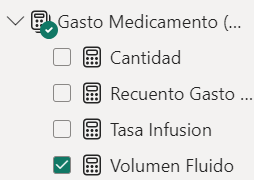
\includegraphics[width=0.4\linewidth]{images/seleccion5-1.png}
		\caption{Creación de un nuevo proyecto multidimensional en Visual Studio.}
		\label{fig:seleccion51}
	\end{center}
\end{figure}

\begin{figure}[H]
	\begin{center} 
		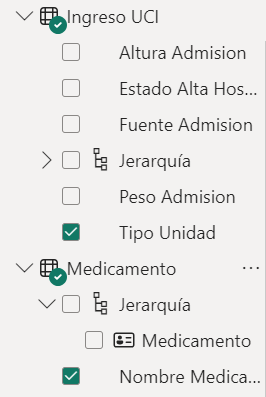
\includegraphics[width=0.35\linewidth]{images/seleccion5-2.png}
		\caption{Creación de un nuevo proyecto multidimensional en Visual Studio.}
		\label{fig:seleccion52}
	\end{center}
\end{figure}

\begin{figure}[H]
	\begin{center} 
		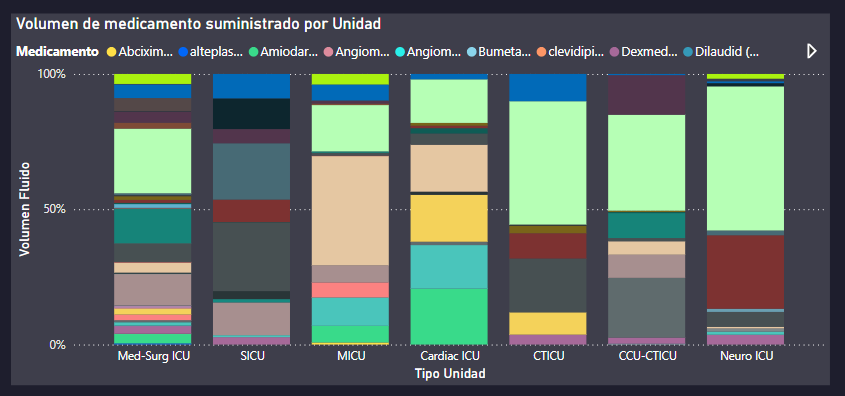
\includegraphics[width=0.7\linewidth]{images/tabla5.png}
		\caption{Creación de un nuevo proyecto multidimensional en Visual Studio.}
		\label{fig:tabla5}
	\end{center}
\end{figure}

\begin{lstlisting}[style=ddlstyle, label=lst:consulta1,caption=Consulta 1: Ranking de Hospitales según Volumen de Fluido]
	
	
SELECT
	nonempty([Ingreso UCI].[Tipo Unidad].Children) ON COLUMNS,
	NONEMPTY(
		[Medicamento].[Nombre Medicamento].Children,
		[Measures].[Volumen Fluido]
	) ON ROWS
FROM 
	[UCIDW]
WHERE 
	[Measures].[Volumen Fluido]
	
\end{lstlisting}

\begin{figure}[H]
	\centering
	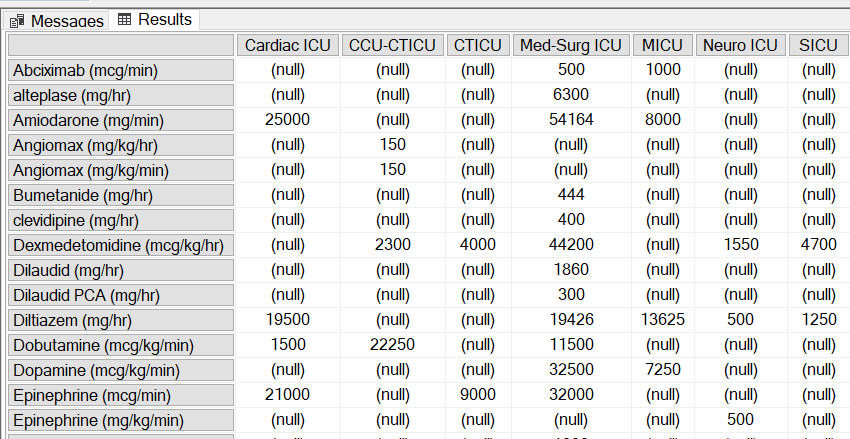
\includegraphics[width=0.65\linewidth]{images/consulta5.png}
	\caption{Resultados de la consulta 1: Ranking de Hospitales según Volumen de Fluido}
	\label{fig:consulta5}
\end{figure}

\subsection{Gráfica 6}

\textbf{Ranking de Hospitales según Volumen de Fluido}
\\

explicar y cambiar titulos
\\

\begin{figure}[H]
	\begin{center} 
		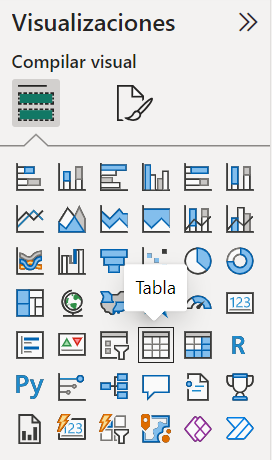
\includegraphics[width=0.35\linewidth]{images/tipo6.png}
		\caption{Creación de un nuevo proyecto multidimensional en Visual Studio.}
		\label{fig:tipo6}
	\end{center}
\end{figure}

\begin{figure}[H]
	\begin{center} 
		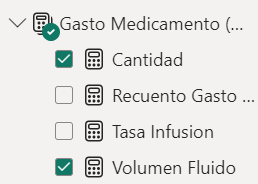
\includegraphics[width=0.4\linewidth]{images/seleccion6-1.png}
		\caption{Creación de un nuevo proyecto multidimensional en Visual Studio.}
		\label{fig:seleccion61}
	\end{center}
\end{figure}

\begin{figure}[H]
	\begin{center} 
		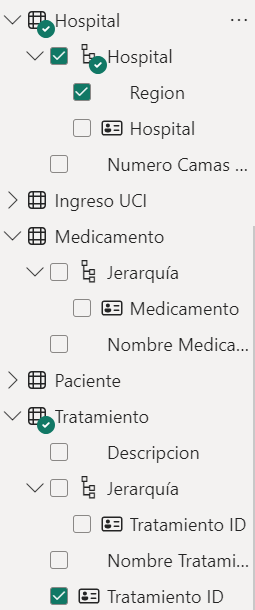
\includegraphics[width=0.35\linewidth]{images/seleccion6-2.png}
		\caption{Creación de un nuevo proyecto multidimensional en Visual Studio.}
		\label{fig:seleccion62}
	\end{center}
\end{figure}

\begin{figure}[H]
	\begin{center} 
		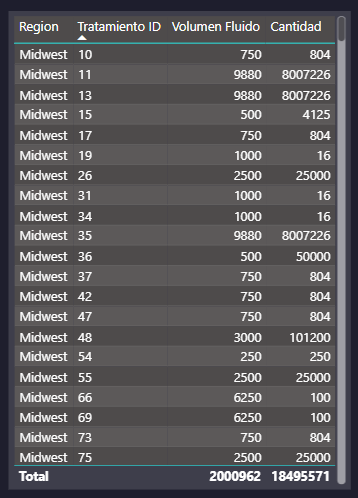
\includegraphics[width=0.5\linewidth]{images/tabla6.png}
		\caption{Creación de un nuevo proyecto multidimensional en Visual Studio.}
		\label{fig:tabla6}
	\end{center}
\end{figure}

\begin{lstlisting}[style=ddlstyle, label=lst:consulta1,caption=Consulta 1: Ranking de Hospitales según Volumen de Fluido]
	
	
SELECT 
	{
		[Measures].[Volumen Fluido],
		[Measures].[Cantidad]
	} ON COLUMNS,
	NONEMPTY(
		CROSSJOIN(
			[Hospital].[Region].Members, 
			[Tratamiento].[Tratamiento ID].Members
		)
	) ON ROWS
FROM 
	[UCIDW]
	
\end{lstlisting}

\begin{figure}[H]
	\centering
	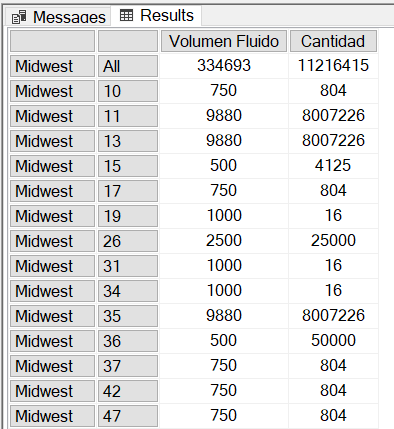
\includegraphics[width=0.4\linewidth]{images/consulta6.png}
	\caption{Resultados de la consulta 1: Ranking de Hospitales según Volumen de Fluido}
	\label{fig:consulta6}
\end{figure}

\section{Tutorial ejecutar consultas}

 \section{Conclusión}
	 \label{sec:conclusion}
	 
	 La creación del cubo multidimensional de gasto de medicamento ha representado un paso clave en nuestro trabajo, construyendo sobre la base sólida establecida por el proceso ETL previo. Este proyecto no solo ha permitido estructurar los datos de manera más intuitiva y accesible, sino que también ha facilitado un análisis más profundo y específico del gasto farmacéutico.
	 
	 En conclusión, el cubo multidimensional desarrollado no solo ofrece una herramienta potente para el análisis del gasto de medicamentos, sino que también representa un avance importante en la construcción de infraestructuras de datos hospitalarios más robustas y orientadas al análisis avanzado.
	 
	\newpage
	\section{Acceso al Repositorio}
	
	Toda la información adicional, incluyendo el código fuente y la documentación completa de este proyecto, está disponible en el repositorio de GitHub \cite{silva2024github}.
	
	% Incluir la bibliografía
	\bibliographystyle{plain}  % Estilo de la bibliografía (por ejemplo, plain, alpha, ieee, etc.)
	\bibliography{bibli}  % Nombre del archivo .bib sin la extensión
	
\end{document}
